\section{Case Study}
\label{sec:casestudy}

In modern distributed computing frameworks (e.g. MPI and ZooKeeper), \emph{leader election} plays an important role to organize multiple servers efficiently and consistently. This section shows how a classical leader election algorithm is modeled and easily used to coordinate other components in \lang{}.

 \cite{HagitDistributed2004} proposed an classical algorithm for a typical leader election scenario, as shown in Figure. \ref{fig:leaderelection}. Distributed processes are organized as a \emph{asynchronous unidirectional} ring where communication take place only between adjacent processes and following certain direction (from left to right in this case).

\begin{figure}
	\centering
	\resizebox{.8\textwidth}{!}{
        \tikzstyle{node}=[
    circle,
    draw
]

\begin{tikzpicture}[remember picture]
    \def \n {5}
    \def \radius {2cm}
    \def \margin {11} % margin in angles, depends on the radius

    \foreach \s in {1,...,\n}
    {
    \node[draw, circle] at ({360/\n * (\s - 1)}:\radius) {$P_\s$};
    \draw[<-, >=latex] ({360/\n * (\s - 1)+\margin}:\radius) 
        arc ({360/\n * (\s - 1)+\margin}:{360/\n * (\s)-\margin}:\radius);
    }

    \node[draw, rectangle, minimum width=4cm] at (6,0) {
        \begin{tabular}{c}
            \\
            Process ($P_i$) \\
             \\
            \begin{tikzpicture}[remember picture]
                \node [draw, rectangle, minimum width=3cm, minimum height=1cm] (connector) at (0,0) {\texttt{election\_module}};
            \end{tikzpicture} \\
            \\
            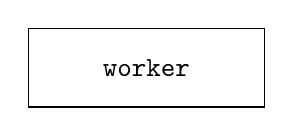
\begin{tikzpicture}[remember picture]
                \node [draw, rectangle, minimum width=3cm, minimum height=1cm] (component) at (0,0) {\texttt{worker}};
            \end{tikzpicture}
            \vspace{0.5em}
        \end{tabular}
        };
    
    \draw[->, >=latex] (3,0.3) -- (connector) node[midway, above, xshift=-0.35cm] {\texttt{left}} ;
    \draw[->, >=latex] (connector) -- (9,0.3) node[midway, above, xshift=0.3cm] {\texttt{right}};
    \draw[<->, >=latex] (component) -- (connector) ;

    \node[] at (0,-2.8) {(a)};
    \node[] at (6,-2.8) {(b)};
\end{tikzpicture}
    }
	\caption{(a) Topology of a Asynchronous Ring and (b) Structure of a Process}
	\label{fig:leaderelection}
\end{figure}

The algorithm mainly includes the following steps:
\begin{enumerate}
	\item To begin with, each process sends a voting message including its own \emph{id} to its successor.
	\item A process, when receives a voting message, will
	\begin{itemize}
		\item forward the message to its successor if it contains a larger \emph{id} than itself,
		\item ignore the message if it contains a smaller \emph{id} than itself, and
		\item take itself as a leader if it contains the same \emph{id} with itself.
	\end{itemize} 
\end{enumerate}

Here we formalize this algorithm through a more general approach. Leader election is encapsulated as \texttt{connector} since it is also responsible to handle the communication between processes. A computing module \texttt{main} is attached to the connector, and used to model computing tasks. 

Two types of messages, \texttt{msgVote} and \texttt{msgLocal}, are supported when formalizing this architecture.
\begin{example}[Definition of Message Types]
Voting messages \texttt{msgVote} are transferred between the connectors. A voting message carries two fields, \emph{vtype} that declares the stage of leader election (either it is still voting or some process has already been acknowledged) and a \emph{id} an identifier of the current leader (if have).
\begin{lstlisting} 
typedef struct { vtype: enum {vote, ack}, id: int } as msgVote;
typedef struct {
	status : enum { pending, acknowledged },
	idLocal : int,
	idLeader : int | NULL
} as msgLocal;
\end{lstlisting}
\end{example}


\begin{lstlisting}
automaton <id:int> election_module (
	left  : in msgVote,  right  : out msgVote,
	query : in msgLocal, notice : out msgLocal
) { ... }

system cluster_instance() {
	components {
		E1 : election_module<1>; E2 : election_module<2>;
		E3 : election_module<3>;
		C1, C2, C2 : worker;
	}	
	connections {
		Sync<msgVote>(E1.left,  E2.right);
		Sync<msgVote>(E2.right, E3.left );
		Sync<msgVote>(E3.right, E1.left );
		
		Sync<msgLocal>(C1,query,  E1.query );
		Sync<msgLocal>(C1,notice, E1.notice);
		Sync<msgLocal>(C2,query,  E2.query );
		Sync<msgLocal>(C2,notice, E2.notice);
		Sync<msgLocal>(C3,query,  E3.query );
		Sync<msgLocal>(C3,notice, E3.notice);
	}
}
\end{lstlisting}